\documentclass[12pt]{article}
\usepackage{float}
\usepackage[table,xcdraw]{xcolor}
\usepackage{tikzit}
\input{Homework.tikzstyles}
\usepackage{hyperref}
\usepackage{amsmath}
\usepackage{amsfonts}
\usepackage{amssymb}
\usepackage{amsthm}
\usepackage{graphics}
\usepackage{graphicx}
\usepackage{yfonts}
\usepackage{float}
\usepackage{dsfont}
\usepackage[nottoc]{tocbibind}
\setcounter{tocdepth}{3}
\setcounter{secnumdepth}{3}
\usepackage{url}
\usepackage{multirow}
\usepackage{subcaption}
\usepackage{ctable}
\usepackage{caption}
\usepackage{pifont}
\usepackage{array}
\usepackage{adjustbox}
\usepackage{booktabs}
\captionsetup{labelformat=empty,labelsep=none}

\title{\textbf{\Luge MRI-Based Brain Tumor Detection}\\[1ex]  Brain Tumor Classification Using CNN}
\author{\Large{ Mohammad Zamani}  \\ \Large{Student No. 610399135} \\ \\ \Large{University of Tehran- CS Department}}
\date{}

\usepackage{titling}
\renewcommand\maketitlehooka{\null\mbox{}\vfill}
\renewcommand\maketitlehookd{\vfill\null}

\begin{document}
	%%%%%%%%%%%%%%%%%%%%%       Title Page      %%%%%%%%%%%%%%%%%%%%%%		

	
	\begin{titlingpage}
	
	\begin{figure}
		\centering
		
\includegraphics[width=0.3\textwidth]{Figs/University_of_Tehran_logo.png}		
	\end{figure}
		\maketitle
	
	\end{titlingpage}
		
	


	%%%%%%%%%%%%%%%%%%%%%       Page 1       %%%%%%%%%%%%%%%%%%%%%%

	\setlength{\parindent}{20pt}
	\tableofcontents
	
	\vspace{1\baselineskip}

	\pagebreak
	\section{Abstract}

	Detecting brain tumors in their early stages is crucial. Brain tumors are classified by biopsy, which can only be performed through definitive brain surgery. Computational intelligence-oriented techniques can help physicians identify and classify brain tumors. Herein, I want to use deep learning methods and machine learning approaches for diag- nosing types of tumor, using MRI brain images to enable to detect with high accuracy tumors in early stages. \\
	This study analyzed 3264 MRI brain images, including tumors and healthy brains. Preprocessing and augmentation were applied. Two neural network models were introduced: a 2D CNN and a convolutional auto-encoder. Both were pretrained with specific hyperparameters. The CNN featured multiple layers with batch-normalization, while the auto-encoder integrated encoded representations for classification.


	\section{Introduction}
	
A brain tumor is a growth of cells in the brain or near it. Brain tumors can happen in the brain tissue. Brain tumors also can happen near the brain tissue. Nearby locations include nerves, the pituitary gland, the pineal gland, and the membranes that cover the surface of the brain.
tumors are known as malignant or benign neoplasms, of which there are more than 200 diverse varieties that may afect humans. According to the American Cancer Society, a brain tumor is a
severe disease in which irregular brain tissue growth
impairs brain function. Te National Brain Tumor Foundation (NBTF) reported that the number of people who have lost their lives due to brain tumors has increased
by 300\% in the last three decades  Te complexity of brain
tumors poses challenges for healthcare providers in diagnosing and caring for afected patients. Early detection of brain tumors and initiation of treatment play vital roles in the survival rate of these patients. Brain tumor biopsy is not as easy as biopsy of other parts of the body, as it must be performed with surgery. Terefore, the need for another method for accurate diagnosis without surgery is crucial. Magnetic Resonance Imaging (MRI) is the best and most commonly used option for diagnosing brain tumors.

The evolution of brain tumor detection has seen a shift towards neural network-based approaches. Early attempts relied on handcrafted features and basic image processing techniques, yielding limited accuracy. However, the advent of deep learning, notably with models like AlexNet and ResNet, revolutionized image analysis. Convolutional Neural Networks (CNNs) have since become instrumental in developing accurate models for tumor detection from MRI images.

Continued research in this field aims to harness the power of CNNs and transfer learning to enhance diagnostic capabilities further. By leveraging advanced neural network architectures and methodologies, researchers strive to develop robust and efficient models for detecting brain tumors, ultimately improving patient outcomes.
	


	\section{Methodology}
	
	\subsection{Methods}
	Te methodology of the present study is illustrated in Fig.\ref{fig:Methodology}. Major steps in the present study comprise brain tumor dataset selection, pre-processing MRI images, feature extraction, and classifcation by various classifers.
	
\begin{figure}[H]
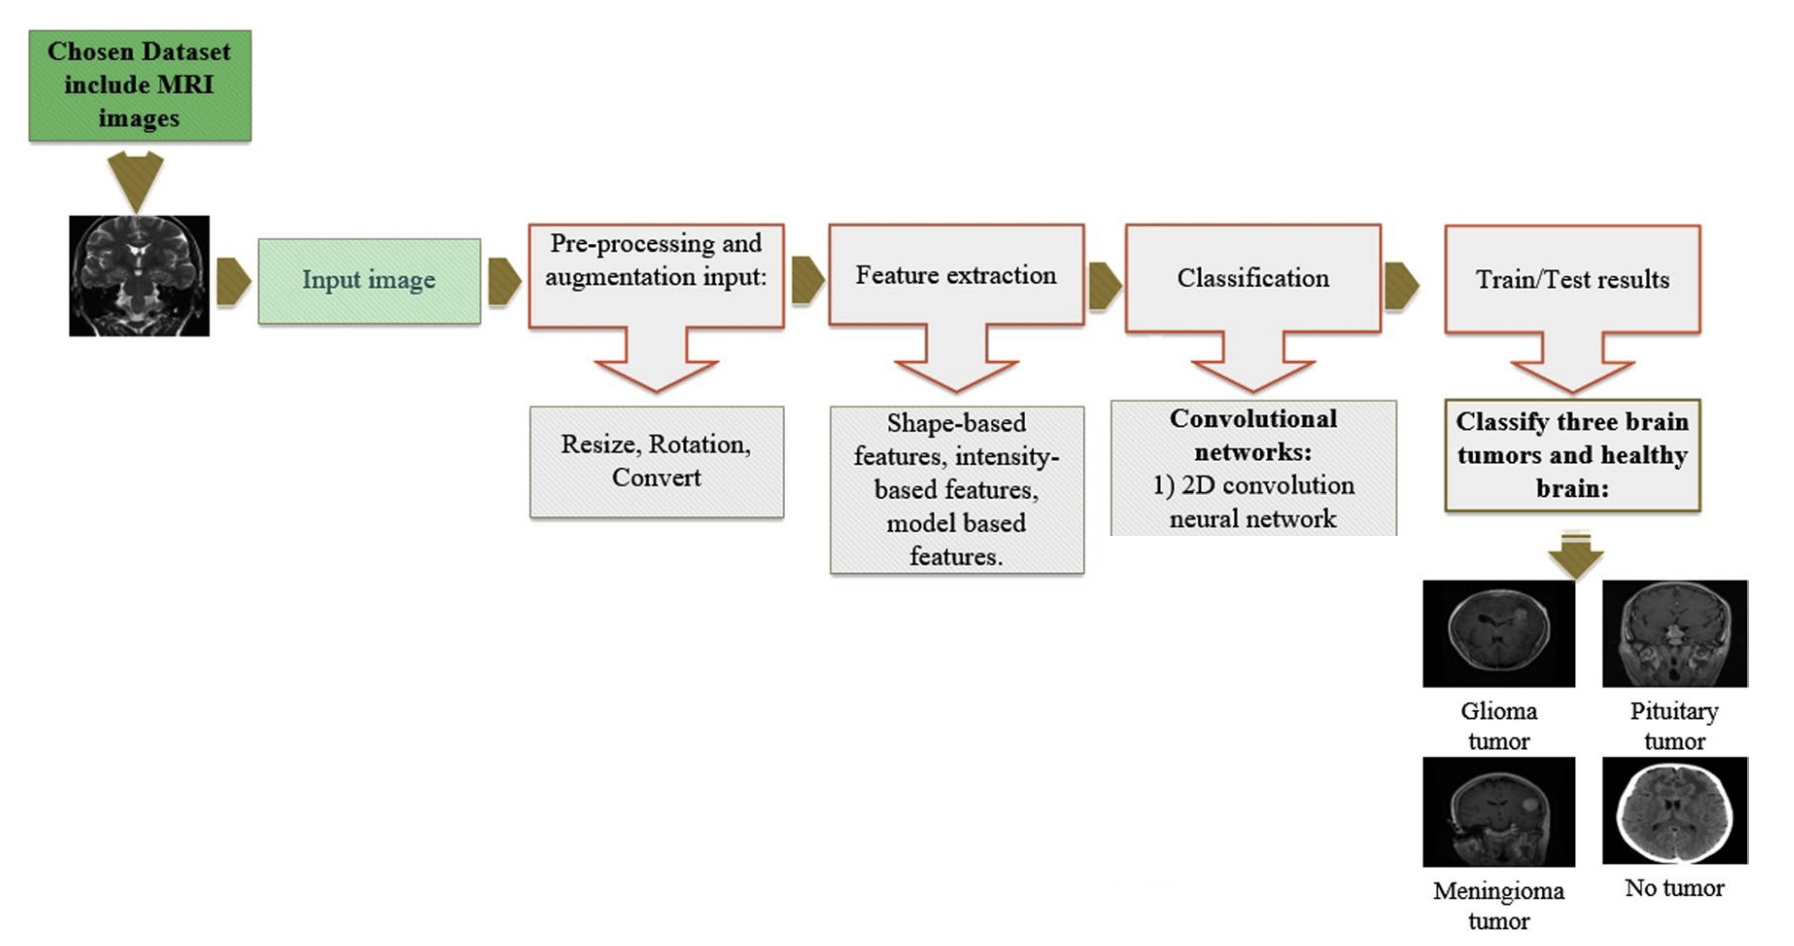
\includegraphics[width=1\textwidth]{Figs/methodology}
\caption{Fig.1 Stages of the proposed methodology}
\label{fig:Methodology}
\end{figure}

	\subsection{Dataset}
	The applied image-based dataset comprised 3264  MRI images.
Tere were four types of images in this dataset: glioma (926 images), meningioma (937 images), pituitary gland tumor (901 images), and healthy brain (500 images). All
images were in sagittal, axial, and coronal planes. Fig.\ref{fig:Dataset} presents examples of the various types of tumors. The number of images is diferent for each patient.


\begin{figure}[H]
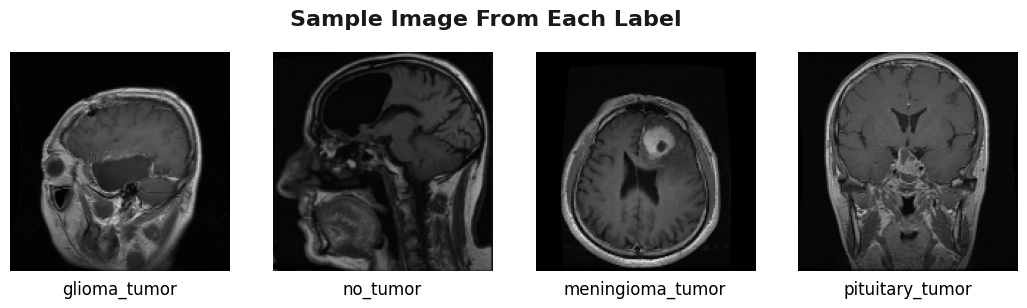
\includegraphics[width=1\textwidth]{Figs/output.png}
\caption{Fig2. MRI samples}
\label{fig:Dataset}
\end{figure}
	
	\subsection{EfficientNetB0}
	EfficientNet is a convolutional neural network architecture and scaling method that uniformly scales all dimensions of depth/width/resolution using a compound coefficient. Unlike conventional practice that arbitrary scales these factors, the EfficientNet scaling method uniformly scales network width, depth, and resolution with a set of fixed scaling coefficients. For example, if we want to use $2^N$
 times more computational resources, then we can simply increase the network depth by $\alpha ^ N$, width by $\beta ^ N$ and image size by $\gamma ^ N$ where $\alpha, \gamma, \beta$
 are constant coefficients determined by a small grid search on the original small model. EfficientNet uses a compound coefficient $\phi$
 to uniformly scales network width, depth, and resolution in a principled way.

The compound scaling method is justified by the intuition that if the input image is bigger, then the network needs more layers to increase the receptive field and more channels to capture more fine-grained patterns on the bigger image.

The base EfficientNet-B0 network is based on the inverted bottleneck residual blocks of MobileNetV2, in addition to squeeze-and-excitation blocks.Fig.\ref{fig:scaling}
 illustrates the difference
between our scaling method and conventional methods.

\begin{center}
\begin{figure}[H]
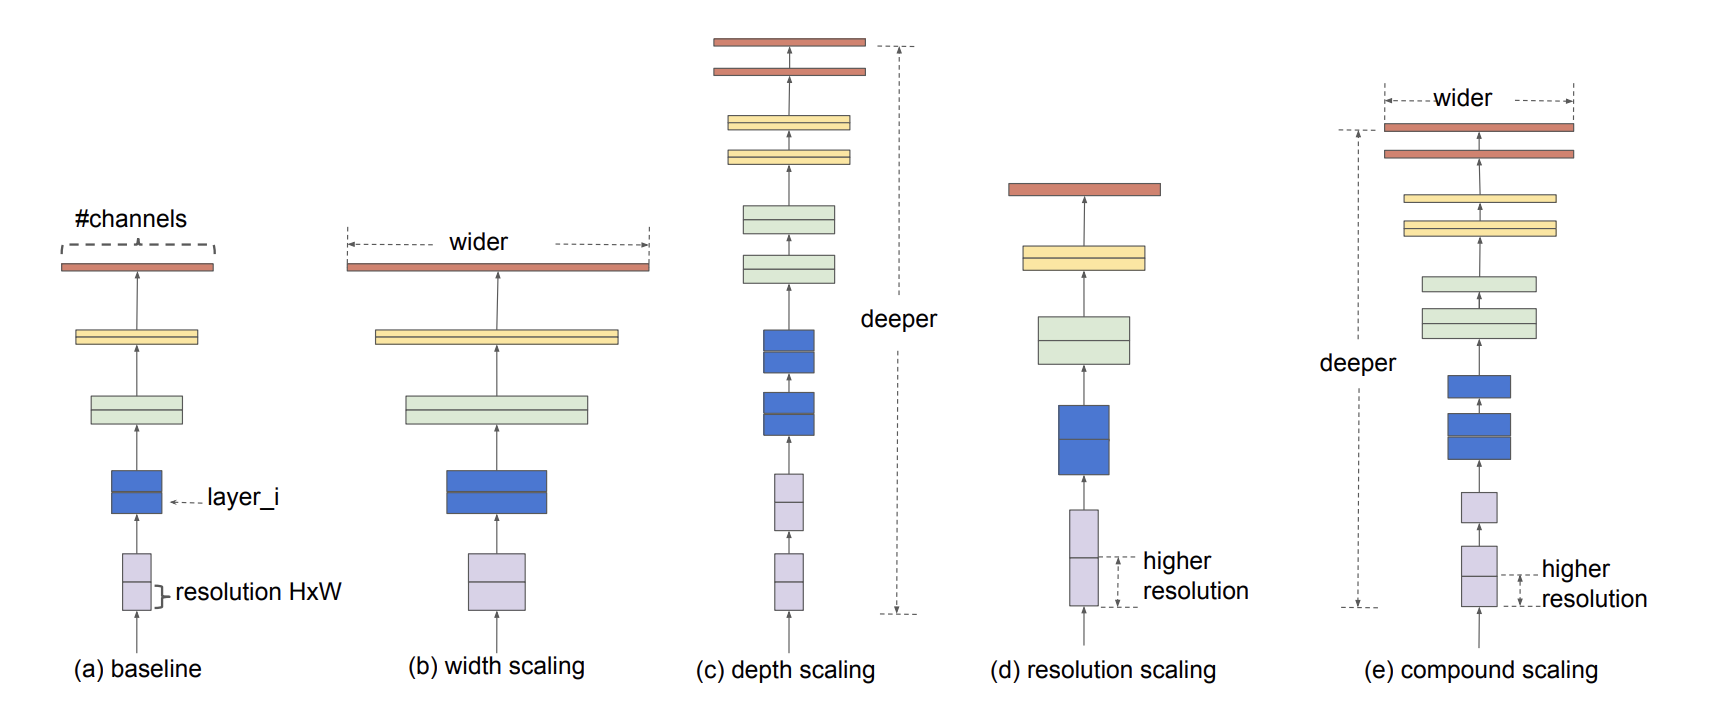
\includegraphics[width=1\textwidth]{Figs/scaling.png}
\caption{Fig.3 \textbf{Model Scaling.} (a) is a baseline network example; (b)-(d) are conventional scaling that only increases one dimension of network width, depth, or resolution. (e) is our proposed compound scaling method that uniformly scales all three dimensions with a fixed ratio.}
\label{fig:scaling}
\end{figure}
\end{center}
	
 Fig.4\ref{fig:effNet} presents the recent EfficientNetB0 baseline model. We propose to use the
EfficientNetB0 baseline model as our entry point that takes in an input image with a
$224 \times 224 \times 3$ dimension. The model then extracts features throughout the layers by using
multiple convolutional (Conv) layers using a $3 \times 3$ receptive field and the mobile inverted
bottleneck Conv (MBConv). Our intuition to employ the EfficientNetB0 is due to its balanced
depth, width, and resolution that can produce a scalable yet accurate and easily deployable
model. Compared to other DCNNs, EfficientNetB0 scales each dimension using a fixed set of
scaling coefficients. This approach surpassed other state-of-the-art models that trained on the
ImageNet dataset. Even with transfer learning, EfficientNet still achieved exceptional results,
indicating its effectiveness beyond the usual ImageNet dataset. In its release, the model had
scales of 0 to 7, showing an increase of parameter size and even accuracy. With the recent
EfficientNet, users and developers can access and provide improved ubiquitous computing
imbued with DL capabilities in several platforms for various needs.

\begin{center}
\begin{figure}[H]
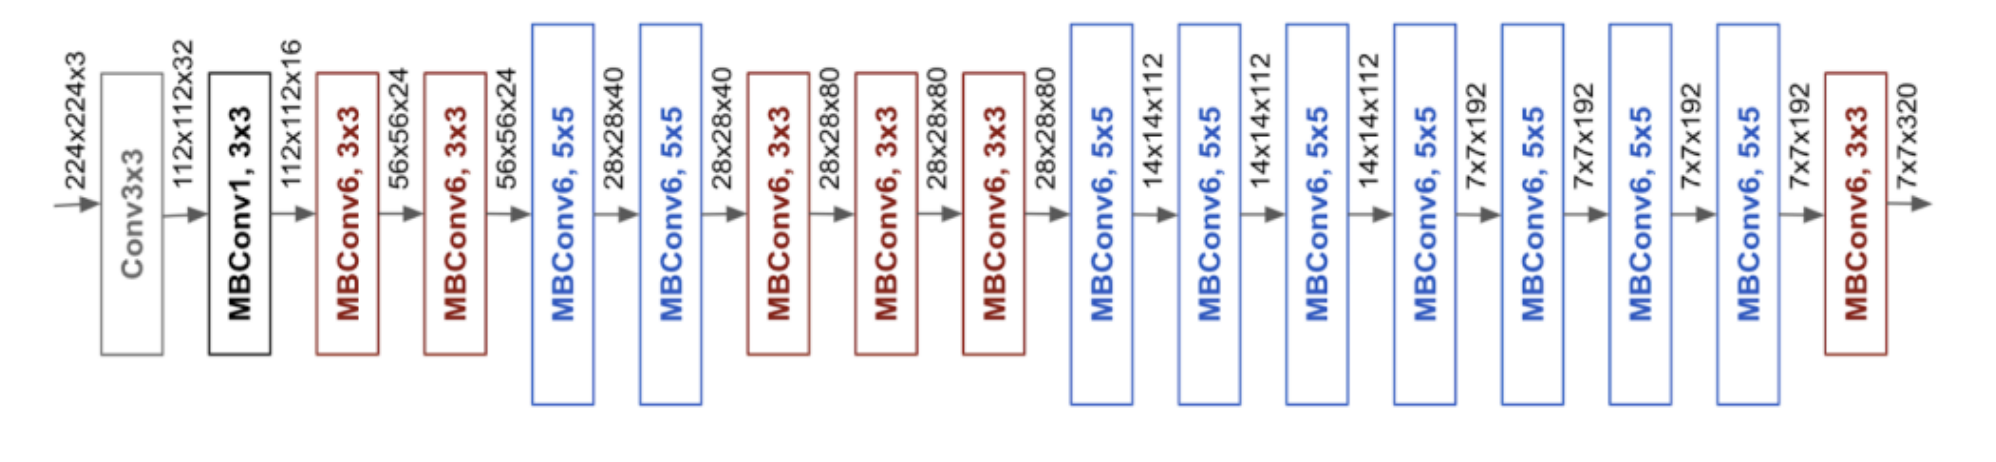
\includegraphics[width=1\textwidth]{Figs/effNet}
\caption{Fig.4 EfficientNetB0 baseline model architecture}
\label{fig:effNet}
\end{figure}
\end{center}
	
	\subsection{Transfer learning}
	
	Deep convolutional neural network models may take days or even weeks to train on very large datasets.
A way to shortcut this process is to reuse the model weights from pre-trained models developed for standard computer vision benchmark datasets, such as the ImageNet image recognition tasks. Top-performing models can be downloaded and used directly or integrated into a new model for your own computer vision problems.
In this project, I'll be using the EfficientNetB0 model, which will utilize the weights from the ImageNet dataset.
so in this step we design the last layer for our purpose.
\begin{table}[ht]
\centering
\begin{tabular}[t]{ccccc}
\hline
Layer & Filter & Kernel Size & Activation\\
\hline
EfficientNetInput (150, 150) & - & - & -\\
GlobalAveragePooling2D & - & - & - \\
Dropout & 0.5 & - & - \\
Dense & 4 & - & softmax \\
\hline
\end{tabular}
\caption{Last layer design.}
\end{table}%


	\section{Results}
	
	\subsection{Training Results}
	The accuracy and loss graphs against the various iterations calculated with the Cross-Entropy (CE) loss are presented in Fig.\ref{fig:training}. The proposed model's training and validation accuracy exhibited a rapid increase within a short period with the given hyper-parameter values. However, the validation accuracy plateaued at around 96\% to 97\%, indicating a limitation in further improvement.

\begin{center}
\begin{figure}[H]
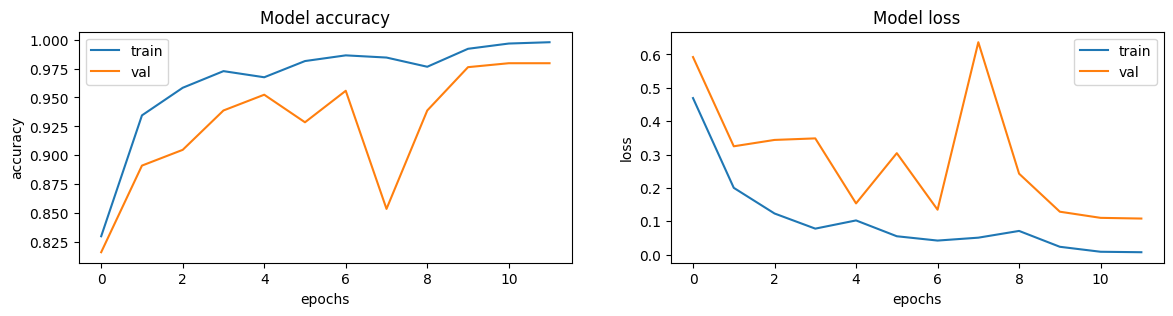
\includegraphics[width=1\textwidth]{Figs/training.png}
\caption{Fig.5 Train and validation trends of the proposed model}
\label{fig:training}
\end{figure}
\end{center}

In the 12 epochs displayed, both the training and validation trends exhibit a logical pattern: decreasing loss and increasing accuracy. This suggests that our training process is proceeding as expected, indicating readiness for evaluation with the test set.

	\subsection{Test Results}
	In ML or DL, the Confusion Matrix (CM) is a standard tool that visualizes how accurate a
trained model can predict from a respective validation dataset. The CM has corresponding
rows and columns representing the actual class and the ground truth labels, consisting of a
parasitized, uninfected blood cells. Simultaneously, the predicted values indicate the number
of correct and incorrect predictions or classifications made for each validation sample. The
True Positive (TP) denotes the number of correctly classified positive samples as positive,
while True Negatives (TN) corresponds to the correctly predicted negatives as negatives. False
Positives (FP) are predictions where the image was classified as positive but is not. In contrast,
False Negatives (FN) are negative results but are positive.
With the following values, we computed for the overall accuracy, precision (PR),
sensitivity (SE), specificity (SP), and the F1-score of each model. In this work, SE signifies
the ratio of correctly predicted parasitized cells or TPs to all TPs and FNs, while SP refers to
the other way around. PR is the frequency of how often the model makes a correct prediction
of an actual class. The accuracy is the total of all accurate predictions out of all the given
samples. At the same time, F1-score is the weighted average between PR and SE.

The following performance metrics are calculated based on the given equations below.
\\
\begin{center}
\begin{equation}
Precision = \frac{TP}{(TP + FP) }
\end{equation} 

 \begin{equation}
Recall = \frac{TP}{(TP + FN) }
\end{equation} 

\begin{equation}
Accuracy = \frac{(TP + TN)}{(TP+ TN + FP + FN)  }
\end{equation} 


\begin{equation}
F1-Score = \frac{ 2TP}{(2TP + FP + FN) }
\end{equation} 
\end{center}
	
	\begin{center}
\begin{figure}[H]
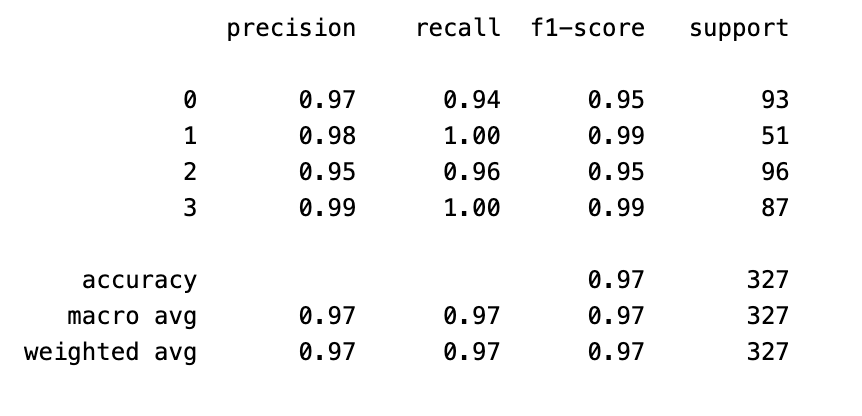
\includegraphics[width=1\textwidth]{Figs/pr}
\caption{Fig.6 Test performance result}
\end{figure}
\end{center}


\begin{center}
\begin{figure}[H]
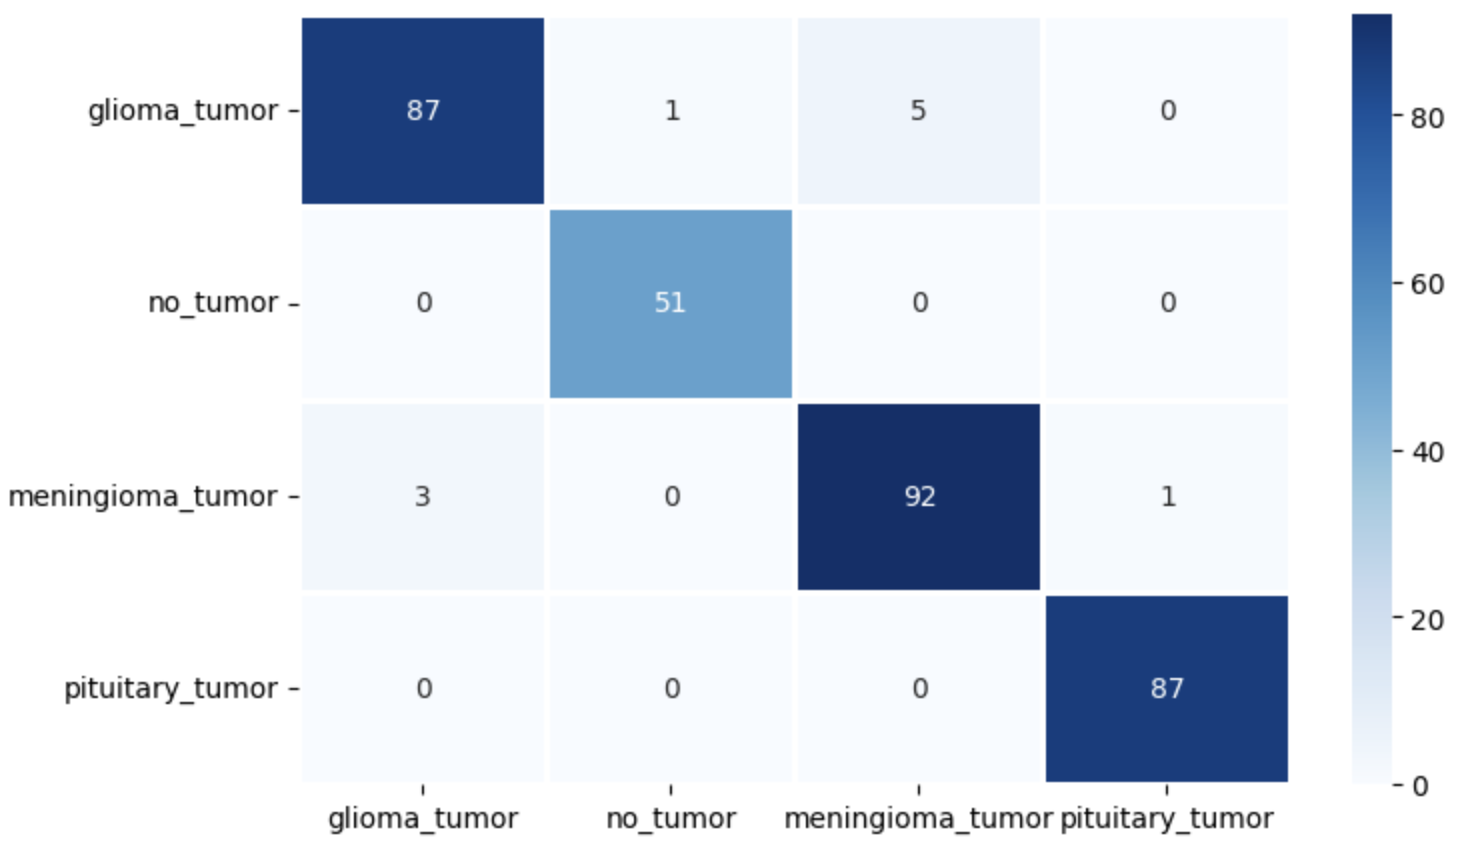
\includegraphics[width=0.8\textwidth]{Figs/CM2}
\caption{Fig.7 Confusion matrix}
\label{fig:CM}
\end{figure}
\end{center}

Fig.\ref{fig:CM} is the result of the confusion matrix of our model, it can be concluded that in the glioma tumor class there are 87  image  data  that  are  predicted  to  be  correct  and  3 image   data   are   predicted   to   be   incorrect,   in   the meningioma tumor class there are 92 image data that are predicted correctly and   5 image predicted incorrectly, in the no tumor class there were 51 image data that were predicted to be correct and 1 image 
data  was  predicted  to  be  incorrect,  and  in  the  pituitary tumor class there were 87 image data that were predicted to  be  correct  and  1  image  data  were  predicted  to  be incorrect.

	\section{Conclusion}
	
In conclusion, the utilization of Convolutional Neural Networks (CNNs), particularly employing the EfficientNet B0 model, has demonstrated remarkable efficacy in the classification of MRI images. Achieving a remarkable accuracy of 97\% underscores the robustness and effectiveness of this approach in accurately identifying and categorizing MRI data. This success not only highlights the potential of deep learning techniques in medical image analysis but also underscores the significance of leveraging state-of-the-art models like EfficientNet B0 for enhanced diagnostic accuracy and efficiency. Moving forward, further exploration and refinement of CNN architectures hold promise for advancing the field of medical image classification, ultimately contributing to improved diagnostic outcomes and patient care in clinical settings.

%%%%%%%%%%%%%%%%%%%%%%%%%%%%%%%%%%%%%%%%%%%%%%%%%%%%%%%%%%%%%%%%%%%%%%%%%%%%%%%%%%%%%%%%%%%%%%%

		%%%%%%%%%%%%%%%%    References    %%%%%%%%%%%%%%%%%%%
	
	
	\begin{thebibliography} {1} % Replace '9' with the widest label in your citations
		\bibitem{MRI-based brain tumor detection using convolutional deep learning methods
and chosen machine learning techniques}MRI-based brain tumor detection using convolutional deep learning methods and chosen machine learning techniques. Soheila Saeedi
, Sorayya Rezayi, Hamidreza Keshavarz and Sharareh R. Niakan Kalhori. 16 January 2023.
		
		\bibitem{CNN Based Multiclass Brain Tumor Detection Using Medical Imaging } CNN Based Multiclass Brain Tumor Detection Using Medical Imaging. Pallavi Tiwari, Bhaskar Pant, Mahmoud M. Elarabawy.  21 June 2022.
		
		\bibitem{Empirical Analysis of a Fine-Tuned Deep Convolutional Model in Classifying and Detecting Malaria Parasites from Blood Smears}Empirical Analysis of a Fine-Tuned Deep Convolutional Model in Classifying and Detecting Malaria Parasites from Blood Smears. Francis Jesmar P. Montalbo and Alvin S. Alon. December 19, 2020.
	
		\bibitem{EfficientNet: Rethinking Model Scaling for Convolutional Neural Networks} EfficientNet: Rethinking Model Scaling for Convolutional Neural Networks. Mingxing Tan, Quoc V. Le. 11 Sep 2020
		
		\bibitem{ Learning augmentation policies
from data}Cubuk, E. D., Zoph, B., Mane, D., Vasudevan, V., and Le,
Q. V. Autoaugment: Learning augmentation policies
from data. CVPR, 2019.
		
		\bibitem{Classification of Brain Tumors on MRI Images Using Convolutional Neural Network Model EfficientNet}Muhammad Aji Purnama Wibowo, Muhammad Bima Al Fayyadl, Yufis Azhar, Zamah Sari. Classification of Brain Tumors on MRI Images Using Convolutional Neural Network Model EfficientNet. Vol. 6 No. 4(2022) 538-547
		
		\bibitem{Brain tumor intro - Mayo Clinic} \href{https://www.mayoclinic.org/diseases-conditions/brain-tumor/symptoms-causes/syc-20350084} Brain tumor intro - Mayo Clinic

	
	\bibitem{ Introduction To Machine Learning, Dr. SharifiZarChi} \href{https://maktabkhooneh.org/}
	Introduction To Machine Learning. Dr. SharifiZarChi.
	
	\bibitem{ Deep Learning for Vision Systems - Mohamed Elgendy - 2020 } \href{https://www.oreilly.com/library/view/deep-learning-for/9781617296192/} Deep Learning for Vision Systems - Mohamed Elgendy - 2020 
	
	\bibitem{ CS231n: Convolutional Neural Networks for Visual Recognition} \href{https://cs231n.github.io/} CS231n: Convolutional Neural Networks for Visual Recognition

		\bibitem{Brain tumor intro - Mayo Clinic} \href{https://www.mayoclinic.org/diseases-conditions/brain-tumor/symptoms-causes/syc-20350084} Brain tumor intro - Mayo Clinic
	\end{thebibliography}
	
\end{document}